\documentclass[12pt,a4paper,oneside,openany]{memoir} 
% Skabelon af DTU's LaTeX support gruppe, v20090423

\usepackage[utf8]{inputenc} 
%\usepackage[danish]{babel} % danske overskrifter
\usepackage[T1]{fontenc}   % fonte (output)
\usepackage{lmodern}       % vektor fonte
\usepackage{fancybox, graphicx}      % indsættelse af billeder
\usepackage{palatino}      % lækker font
\usepackage{pdfpages}      % pdf som forside evt
\usepackage{todonotes}
\usepackage{microtype}
% \linespread{1.3}           % kræver lidt mere line spacing

\newcommand{\code}[1]{\texttt{#1}}
\newcommand{\HRule}{\rule{\linewidth}{0.5mm}}

%\addto\captionsdanish{
%  \renewcommand{\contentsname}%
%    {Indholdsfortegnelse}     %
%} % Så bruger vi bare 'Indholdsfortegnelse' i stedet for 'Indhold'


\usepackage{underscore}
\usepackage{pdflscape}
\usepackage{todonotes}

\usepackage[plainpages=false,pdfpagelabels,pageanchor=false]{hyperref} % aktive links
\def\sectionautorefname{afsnit}

\usepackage{memhfixc}  % rettelser til hyperref

\usepackage{tipa}
\pretolerance=2500     % højt tal, mindre orddeling og mere space mellem ord.
% 3000 er okey, 1000 er for lidt, 5000 i overkanten, 8000 er for meget..

\usepackage[font=small,labelfont=bf,labelsep=endash]{caption}
 
\pagestyle{headings}


\makechapterstyle{mortenovi}{%
\setlength{\beforechapskip}{0cm}%længde fra top af side til kapitel-overskrifter
\setlength{\afterchapskip}{1cm}%længde fra kapiteltekst til body-tekst
\setlength{\midchapskip}{2cm}%længe mellem kapitelnummer og kapiteltekst
\renewcommand\chapnamefont{\normalfont\Large\scshape\raggedleft}
\renewcommand\chaptitlefont{\normalfont\Huge\bfseries\sffamily}
\renewcommand\chapternamenum{}%default "kapitel"
\renewcommand\printchapternum{%
    \makebox[0pt][l]{%
    \hspace{0.4em}
    \resizebox{!}{4ex}{\chapnamefont\bfseries\sffamily\thechapter}}
    }%"kapitel. x"-linjen og dens boxe og bredder - prøv at sætte xyz ind først på de tre linjer respektivt.
\renewcommand\afterchapternum{\par\hspace{1.5cm}\hrule\vspace{0.5cm}}
\renewcommand\afterchaptertitle{\vskip\onelineskip \hrule\vskip\afterchapskip
}}
\chapterstyle{mortenovi}

\maxtocdepth{subsection} %Only parts, chapters and sections in the table of contents
\settocdepth{subsection}

% \includeonly{forord,testing} % Kompiler kun de kapitler du arbejder med.

\usepackage{listings}
\usepackage{color}

\renewcommand*\lstlistingname{Kode}

\definecolor{dkgreen}{rgb}{0,0.6,0}
\definecolor{gray}{rgb}{0.5,0.5,0.5}
\definecolor{mauve}{rgb}{0.58,0,0.82}

\lstset{frame=tb, %lr
  language=Java,
  aboveskip=3mm,
  belowskip=3mm,
  showstringspaces=false,
  columns=flexible,
  basicstyle={\small\ttfamily},
  numbers=none,
  numberstyle=\tiny\color{gray},
  keywordstyle=\color{blue},
  commentstyle=\color{dkgreen},
  stringstyle=\color{mauve},
  breaklines=true,
  breakatwhitespace=true,
  basicstyle=\tiny\ttfamily
}

\usepackage{cleveref}


\begin{document}
%\includepdf[fitpaper]{billeder/forside}


\begin{center}
\thispagestyle{empty}

% Upper part of the page. The '~' is needed because \\
% only works if a paragraph has started.

\textsc{\LARGE IT University of Copenhagen}\\[1.5cm]

\textsc{\Large BMDS 2014 }\\[0.5cm]

% Title
\HRule \\[0.4cm]
{ \huge \bfseries Designated Exercise Set 1\\ [0.4cm]
    %\large \\ [0.4cm] 
    }

\HRule \\[1cm]

\textsc{\Large Assignment 1 }\\[1.5cm]

% Author and supervisor
\begin{minipage}{1\textwidth}
\begin{center} \large
Anders Wind Steffensen - awis@itu.dk\\
Anders Fischer-Nielsen - afin@itu.dk\\
Christopher Blundell - cnbl@itu.dk\\
Daniel Varab - djam@itu.dk\\
\end{center}
\end{minipage}


\vfill

% Bottom of the page
{\large \today}

\end{center}

\frontmatter%

%\include{abastract}
%\include{preface}

%\tableofcontents* % stjernen betyder vi ikke har den med i vores indholdsfortegnelse


\newpage

\mainmatter%

%input chapters here

\chapter{Answers}
\section{Exercise A.}
A client attempts to synchronise with a time server. It records the round-trip times and timestamps returned by the server in the table below.\\
\begin{itemize}
\item Which of these times should it use to set its clock? 
\item To what time should it set it? 
\item Estimate the accuracy of the setting with respect to the server’s clock. 
\item If it is known that the time between sending and receiving a message in the system concerned is at least 8 ms, do your answers change?
\end{itemize}
\begin{tabular}{ l | r }
Round-trip (ms) & Time (hr:min:sec) \\[0.1cm]
\hline \\
(A) 22 & 10:54:23.674 \\[0.1cm]
(B) 25 & 10:54:25.450 \\[0.1cm]
(C) 20 & 10:54:28.342 \\[0.1cm]
\hline 
\end{tabular}\\\\

\textbf{A.1 - Which of these times should it use to set its clock?}\\
Picking the time which had the fastest round trip (C) gives us a smaller margin for error. This means better accuracy. Therefore the answer is (A) 10:54:23.674. Since we do not know the distribution of the time from and to the server, the smaller the round trip, the smaller the difference is possible.\\

\textbf{A.2 - To what time should it set it?}\\
Since we picked C for setting the time we will use the result to calculate the time using the form
time + (round trip/2)\\
With our data:\\
10:54:28:342+20/2 = 10:54:28:352\\
Therefore we should set the time to 10:54:28:352\\

\textbf{A.3 - Estimate the accuracy of the setting with respect to the server’s clock.}\\
Since we add the roundtrip divided by two to the time, we have some inaccuracy. We are not sure if the first half of the roundtrip might take 0 ms or 20 and the trip back then respectively 20 or 0 ms. Therefore the accuracy of this clock may be 
\begin{quote}
+-(TRound / 2 - min)

With our data (and with min removed since we do not know it):

+-(20ms / 2) = +-10ms
\end{quote}
Therefore the accuracy of our clock will be +-10ms\\

\textbf{A.4 - If it is known that the time between sending and receiving a message in the system concerned is at least 8 ms, do your answers change?}\\

@A.1 - Even if we know that the round trip takes at least 8 ms, it still wouldn’t make sense to pick a less accurate time such as (A) and (B).\\

@A.2 - The answer to our second question would not change either considering we don’t change our answer to the first question.\\

@A.3 - The accuracy of (C) would change to 2 ms since we now know the minimum time we can use the fomular for accuracy one more time
\begin{quote}
+-(TRound / 2 - min)

With our data:

(20ms / 2 - 8) = +-2ms for (C)
\end{quote}
Therefore with a minimum time of 8 ms and using the (C) roundtrip the accuracy of the clock would be 2ms.
\newpage
\section{Exercise B.}
\section{Exercise C.}
Consider this diagram:\\

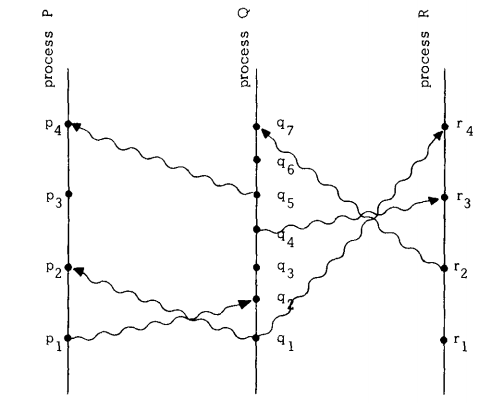
\includegraphics[scale=0.7]{ExerciseC-processDiagram}\\
\begin{enumerate}
\item Write out the happens-before relation in the following diagram. (Immediate successors is fine; you don’t have to write the entire transitive closure.
\item Identify 4 consistent cuts.
\item Identify 4 inconsistent cuts.
\item Write 2 different linearizations of the events in this diagram.
\end{enumerate}

\textbf{1) Happens before successors.}\\
\begin{tabular}{ l r }
\hline \\[0.1cm]
q1->q2->q3->q4->q5->q6->q7 	& HB statement 1 \\[0.1cm]
p1->p2->p3->p4 				& HB statement 1 \\[0.1cm]
r1->r2->r3->r4 				& HB statement 1 \\[0.1cm]
\hline \\[0.1cm]
p1->q2 & HB statement 2 \\[0.1cm]
q1->p2 & HB statement 2 \\[0.1cm]
q1->r4 & HB statement 2 \\[0.1cm]
q4->r3 & HB statement 2 \\[0.1cm]
q5->p4 & HB statement 2 \\[0.1cm]
r2->q7 & HB statement 2 \\[0.1cm]
\hline 
\end{tabular}\\\\

\textbf{2) Consistent cuts}\\
\begin{tabular}{ l l l }
Process P & Procces Q & Process R \\[0.1cm]
\hline 
p1 		& q1 	& r1 	\\[0.1cm]
p1-p3 	& q1-q4 & r1-r4 \\[0.1cm]
p1 		& q1-q7 & r1-r2 \\[0.1cm]
p1-p4 	& q1-q7 & r1-r4 \\[0.1cm]
\hline 
\end{tabular}\\\\

\textbf{2) Inconsistent cuts}\\
\begin{tabular}{ l l l | l }
Process P & Procces Q & Process R & Explanation \\[0.1cm]
\hline 
p1-p4 	& q1 	& r1 	& q5->p4 			\\[0.1cm]
p1-p3 	& q1-q2 & r1-r4 & q4->r3 , vr3-> r4 \\[0.1cm]
p1 		& q1-q7 & r1 	& r2->q7 			\\[0.1cm]
p1-2	& none 	& r1-r4 & q1->p2, q1->r4 	\\[0.1cm]
\hline 
\end{tabular}\\\\

\newpage
\section{Exercise D.}
Two processes P and Q are connected in a ring using two channels, and they constantly rotate a message m. At any one time, there is only one copy of m in the system. Each process’s state consists of the number of times it has received m, and P sends m first. At a certain point, P has the message and its state is 101. Immediately after sending m, P initiates the snapshot algorithm. Explain the operation of the algorithm in this case, giving the possible global state(s) reported by it.\\\\
The snapshot algorithm as described in \emph{Distributed Systems — Concepts \& Design} p. 616\\

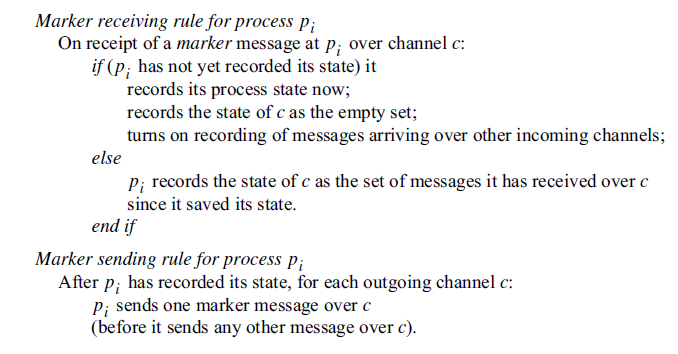
\includegraphics[scale=0.7]{Snapshot-Algorithm}\\

Since P initiates the algorithm we look at the ‘Marker sending rule for process’ first, therefore P records its state to begin with, and since it has received the message M 101 times, this value will be stored. P only has one channel and therefore it sends a marker message along it to Q, and afterwards turns on recording of messages arriving over other incoming channels.

Q at this time receives M and therefore raises its state to 102 and sends the message on again. Shortly after Q receives the Marker message from P and therefore starts the “Marker receiving rule for process”. Since it has not yet recorded its state it does so, and then records the incoming channel as empty. No other incoming channels exists so the algorithm is done.

\newpage
\section{Exercise E.}
Consider this distributed system: There are 3 processes; each process has a state consisting of a single number k. Whenever a process receives a message, it updates its state k to a randomly chosen new number. If the state k of a process is even, it will transmit messages at random intervals; if odd, it does nothing.\\\\
Questions
\begin{enumerate}
\item Explain how this system may deadlock.
\item Explain how this system may deadlock even if you can make no assumptions on the initial state.
\item Explain how the snapshot algorithm can be used to discover if the system has deadlocked. (NB! Assume that a process in odd state will nonetheless send markers as required by the algorithm. Moreover, a process which receives a message containing only a marker does not update its state k.)
\item Summarise the steps of the snapshot algorithm when executed on the system with initial global states 3, 4, 7 and no messages in transit. Will the resulting snapshot allow you to conclude that the system is deadlocked?
\item Summarise the steps of the snapshot algorithm when executed on the system with initial global states 3, 5, 7 and no messages in transit. Will the resulting snapshot allow you to conclude that the system is deadlocked?
\end{enumerate}
Answers
\begin{enumerate}
\item The system will deadlock if all processes are have k as an uneven number. If the system starts with every process with k equal to an uneven number, nothing will happen at all as the system will be locked, unable to retrieve.
\item The system can still freeze. Since every process gets a random number, all three processes might get an uneven number again. Imagine a given point in time where p1 = uneven, p2 = uneven, p3 even. P3 is sendings messages at an unknown interval, which pings p2 whichs random outcome sets its k-value to an even number. Now, simultaneously p3 and p2 send each other a message, which unluckily both result in uneven k-evaluations, effectively deadlocking the system.
\item As the snapshot algorithm can be used to monitor the traffic of a distributed system one may inspect the states to disclose deadlocks. If processes are not omitting messages and the channels are empty it is safe to say that a deadlock has occurred.
\item \emph{S0: p1:<3>, p2:<4>, p3<7>, c1:<>, c2:<>, c3:<>, c4:<>, c5:<>, c6:<>} \\
As the snapshot algorithm is initiated on an empty system the first step is to emit the sending rule by sending a mark from p2 to its outgoing channels (p1 and p3) which are consequently pushed to record their state as a result of the receiving rule. Assuming for the sake of this question, p2 sends its message (m) to process p1 via channel c2 after its mark, p1 will set c2<m> as specified to the algorithm. At this point we are in the final global state which isn’t a deadlock due to the factor of p2s continuation to send messages. This is visible through the snapshot by the state of c<m>.\\
\emph{Final global state: p1:<3>, p2:<4>, p3<7>, c1:<>, c2:<m>, c3:<>, c4:<>, c5:<>, c6:<>}
\item \emph{S0 \& final global state: p1:<3>, p2:<5>, p3<7>, c1:<>, c2:<>, c3:<>, c4:<>, c5:<>, c6:<>} \\
Just as the previous answer, the initial marks will be broadcasted to the different processes, but in contrary there is no message to be sent and we find ourself in the definition of a deadlock: all processes are waiting. This is aligned with the snapshot as it shows that no messages are in any channels.
\end{enumerate}


\end{document}